\documentclass[tikz,border=10pt]{standalone}
\usetikzlibrary{arrows.meta, positioning, decorations.pathmorphing, fit, backgrounds, calc}

\begin{document}
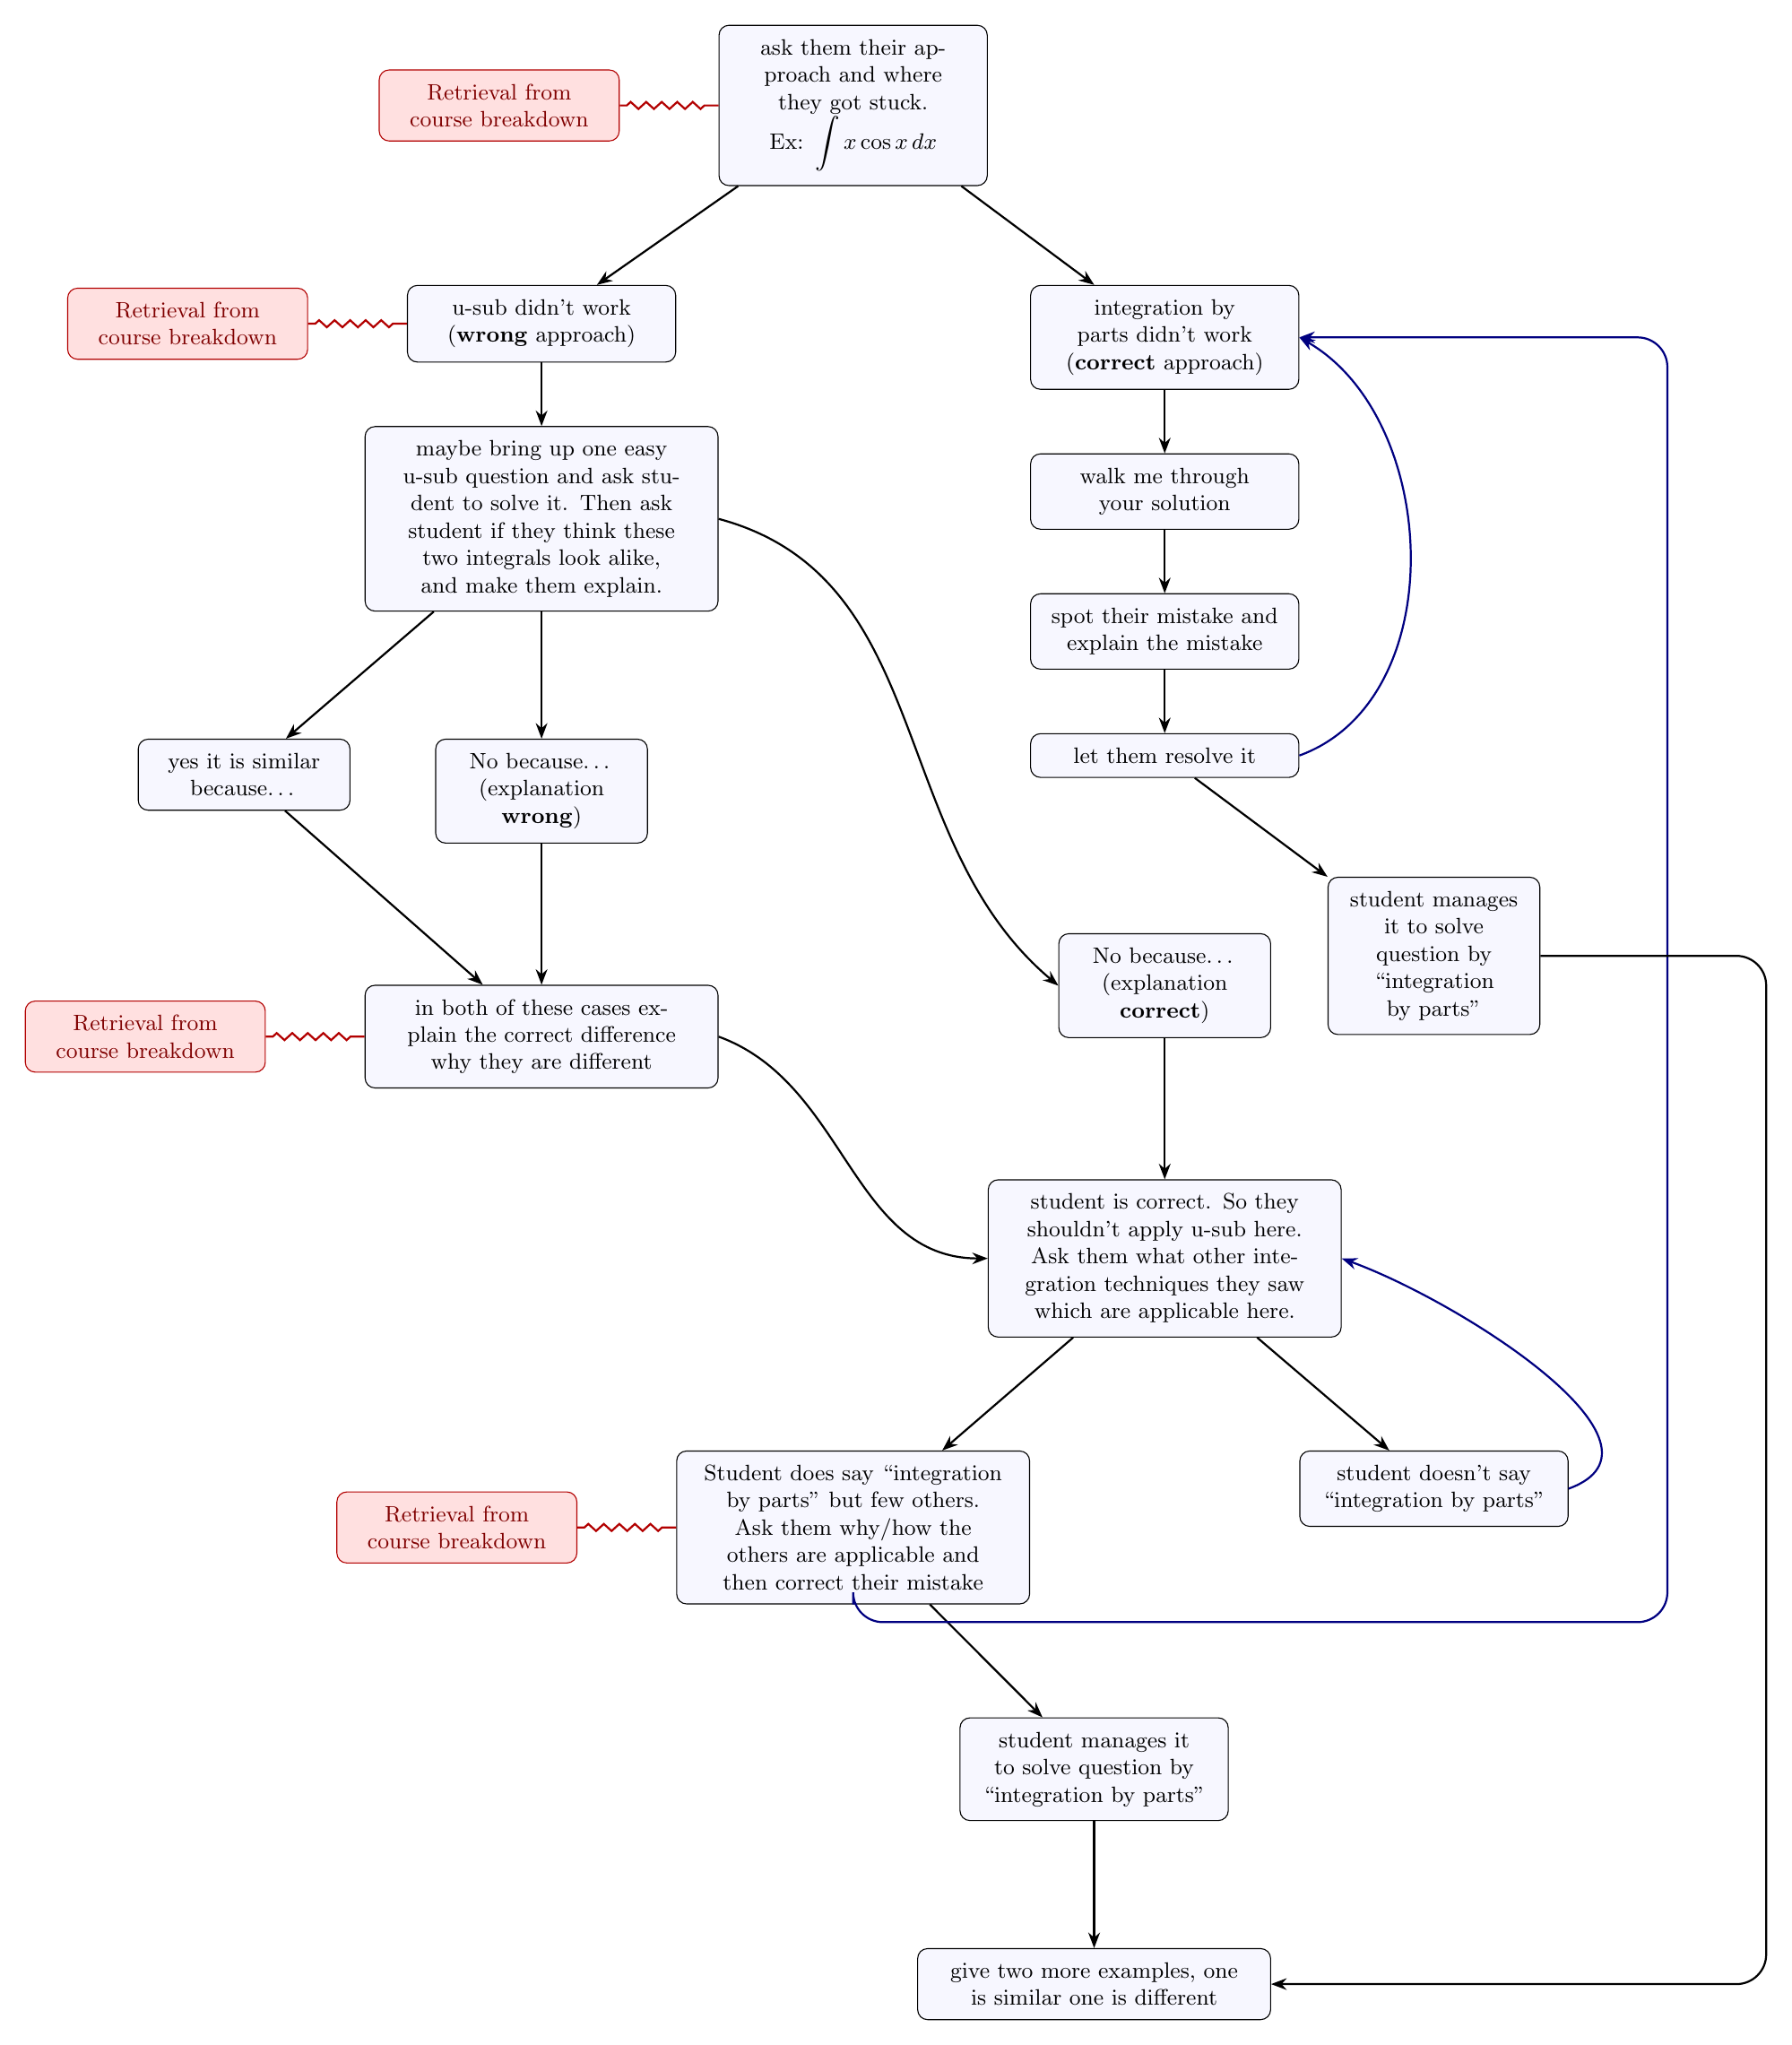
\begin{tikzpicture}[
  font=\small,
  node distance=9mm and 10mm,
  every node/.style={align=center},
  box/.style={draw, rounded corners, align=center, text width=3.4cm, inner sep=2mm, fill=blue!3},
  wide/.style={text width=4.6cm},
  narrow/.style={text width=2.6cm},
  note/.style={draw, dashed, rounded corners, align=left, text width=6cm, inner sep=2mm, fill=yellow!8},
  arr/.style={-{Stealth[length=2.2mm]}, thick},
  wavyarr/.style={-{Stealth[length=2.2mm]}, thick, decorate,
                  decoration={zigzag, segment length=2.2mm, amplitude=0.5mm, pre length=1mm, post length=2mm}},
  loopback/.style={-{Stealth[length=2.2mm]}, thick, blue!50!black},
  % red "retrieval" nodes and their wavy (arrowless) connectors
  retr/.style={draw=red!70!black, rounded corners, align=center, text width=3cm, inner sep=2mm, fill=red!12, text=red!50!black},
  wavy/.style={thick, red!70!black, decorate,
               decoration={zigzag, segment length=2.2mm, amplitude=0.5mm, pre length=1mm, post length=1mm}}
]

% ---------- Root ----------
\node[box] (root) {ask them their approach and where they got stuck. Ex: $\displaystyle\int x\cos x\,dx$};

% ---------- Level 1 ----------
\node[box, below left=14mm and 6mm of root] (usub) {u-sub didn't work (\textbf{wrong} approach)};
\node[box, below right=14mm and 6mm of root] (parts) {integration by parts didn't work (\textbf{correct} approach)};

\draw[arr] (root) -- (usub);
\draw[arr] (root) -- (parts);

% ---------- u-sub branch ----------
\node[box, wide, below=of usub] (usubq) {maybe bring up one easy u-sub
  question and ask student to solve it. Then ask student if they think
  these two integrals look alike, and make them explain.};
\draw[arr] (usub) -- (usubq);

\node[box, narrow, below left=18mm and 2mm of usubq] (usubyes) {yes it is
  similar because\ldots};
\node[box, narrow, below=18mm of usubq] (usubnowrong) {No because\ldots\\
  (explanation \textbf{wrong})};

\node[box, wide, below=20mm of usubnowrong] (usubdiff) {in both
  of these cases explain the correct difference why they are different};

\draw[arr] (usubq) -- (usubyes);
\draw[arr] (usubq) -- (usubnowrong);
\draw[arr] (usubyes) -- (usubdiff);
\draw[arr] (usubnowrong) -- (usubdiff);

% ---------- integration by parts branch ----------
\node[box, below=of parts] (partswalk) {walk me through your solution};
\node[box, below=of partswalk] (partsspot) {spot their mistake and
  explain the mistake};
\node[box, below=of partsspot] (partsresolve) {let them resolve it};

\draw[arr] (parts) -- (partswalk);
\draw[arr] (partswalk) -- (partsspot);
\draw[arr] (partsspot) -- (partsresolve);

\node[box, narrow, below right=14mm and 4mm of partsresolve] (partssolves)
  {student manages it to solve question by ``integration by parts''};
\node[box, narrow, below=22mm of partsresolve] (partsnocorrect)
  {No because\ldots\\ (explanation \textbf{correct})};

\draw[arr] (partsresolve) -- (partssolves);

% if not solved, go back and redo the "walk me through / spot mistake / resolve" steps
\draw[loopback] (partsresolve.east) to[out=20, in=-30] (parts.east);

% merge: the "easy u-sub question" branch's third outcome joins here
\draw[arr] (usubq.east) to[out=-15, in=140] (partsnocorrect.west);

% ---------- merge point ----------
\node[box, wide, below=20mm of partsnocorrect] (correctnode) {student is
  correct. So they shouldn't apply u-sub here. Ask them what other
  integration techniques they saw which are applicable here.};

\draw[arr] (partsnocorrect) -- (correctnode);
\draw[arr] (usubdiff.east) to[out=-20, in=180] (correctnode.west);

\node[box, wide, below left=16mm and -6mm of correctnode] (saysparts)
  {Student does say ``integration by parts'' but few others. Ask them
  why/how the others are applicable and then correct their mistake};
\node[box, below right=16mm and -6mm of correctnode] (notsaysparts)
  {student doesn't say ``integration by parts''};

\draw[arr] (correctnode) -- (saysparts);
\draw[arr] (correctnode) -- (notsaysparts);
\draw[loopback] (notsaysparts.east) to[out=20, in=-20] (correctnode.east);

\node[box, below right=16mm and -10mm of saysparts] (manages)
  {student manages it to solve question by ``integration by parts''};
\draw[arr] (saysparts) -- (manages);

\coordinate (rightChan1) at ($(notsaysparts.east)+(14mm,0)$);

% arrow from "Student does say integration by parts..." back to
% "integration by parts didn't work" (routed around the right side,
% dropping below the "doesn't say" row first so it doesn't cut through that box)
\coordinate (dropY) at ($(notsaysparts.south)!0.5!(manages.north)$);
\draw[loopback, rounded corners=12pt]
  (saysparts.south) -- (saysparts.south |- dropY)
  -- (rightChan1 |- dropY)
  -- (rightChan1 |- parts.east)
  -- (parts.east);

% ---------- final convergence node ----------
\node[box, wide, below=18mm of manages] (twoexamples) {give two more
  examples, one is similar one is different};

\draw[arr] (manages) -- (twoexamples);

% long arrow from the other "student manages it..." node, routed around the
% right side so it doesn't cut through partsnocorrect / correctnode / notsaysparts / manages
\coordinate (rightChan2) at ($(rightChan1)+(14mm,0)$);
\draw[arr, rounded corners=12pt]
  (partssolves.east) -- (rightChan2 |- partssolves.east)
  -- (rightChan2 |- twoexamples.east)
  -- (twoexamples.east);

% ---------- Retrieval-from-course-breakdown nodes (red) ----------
% one red node placed to the left of each of the four target nodes,
% joined by a wavy line with no arrow head
\node[retr, left=14mm of root]      (retr1) {Retrieval from course breakdown};
\node[retr, left=14mm of usub]      (retr2) {Retrieval from course breakdown};
\node[retr, left=14mm of usubdiff]  (retr3) {Retrieval from course breakdown};
\node[retr, left=14mm of saysparts] (retr4) {Retrieval from course breakdown};

\draw[wavy] (retr1.east) -- (root.west);
\draw[wavy] (retr2.east) -- (usub.west);
\draw[wavy] (retr3.east) -- (usubdiff.west);
\draw[wavy] (retr4.east) -- (saysparts.west);

\end{tikzpicture}
\end{document}